\chapter{科技进步}
\label{chapter:technology}
《“十四五”推进农业农村现代化规划》提出\cite{national-agricultural-green-development-plan},计划到2025年,农业基础更加稳固,乡村振兴战略全面推进,农业农村现代化取得重要进展。科技的进步显著推动了乡村发展,不仅改变了农村的面貌,也为乡村振兴注入了新的活力\cite{农办科〔2023〕15号附件}。
以下是十四五规划的规划目标图:
\begin{figure}[h]
    \centering
    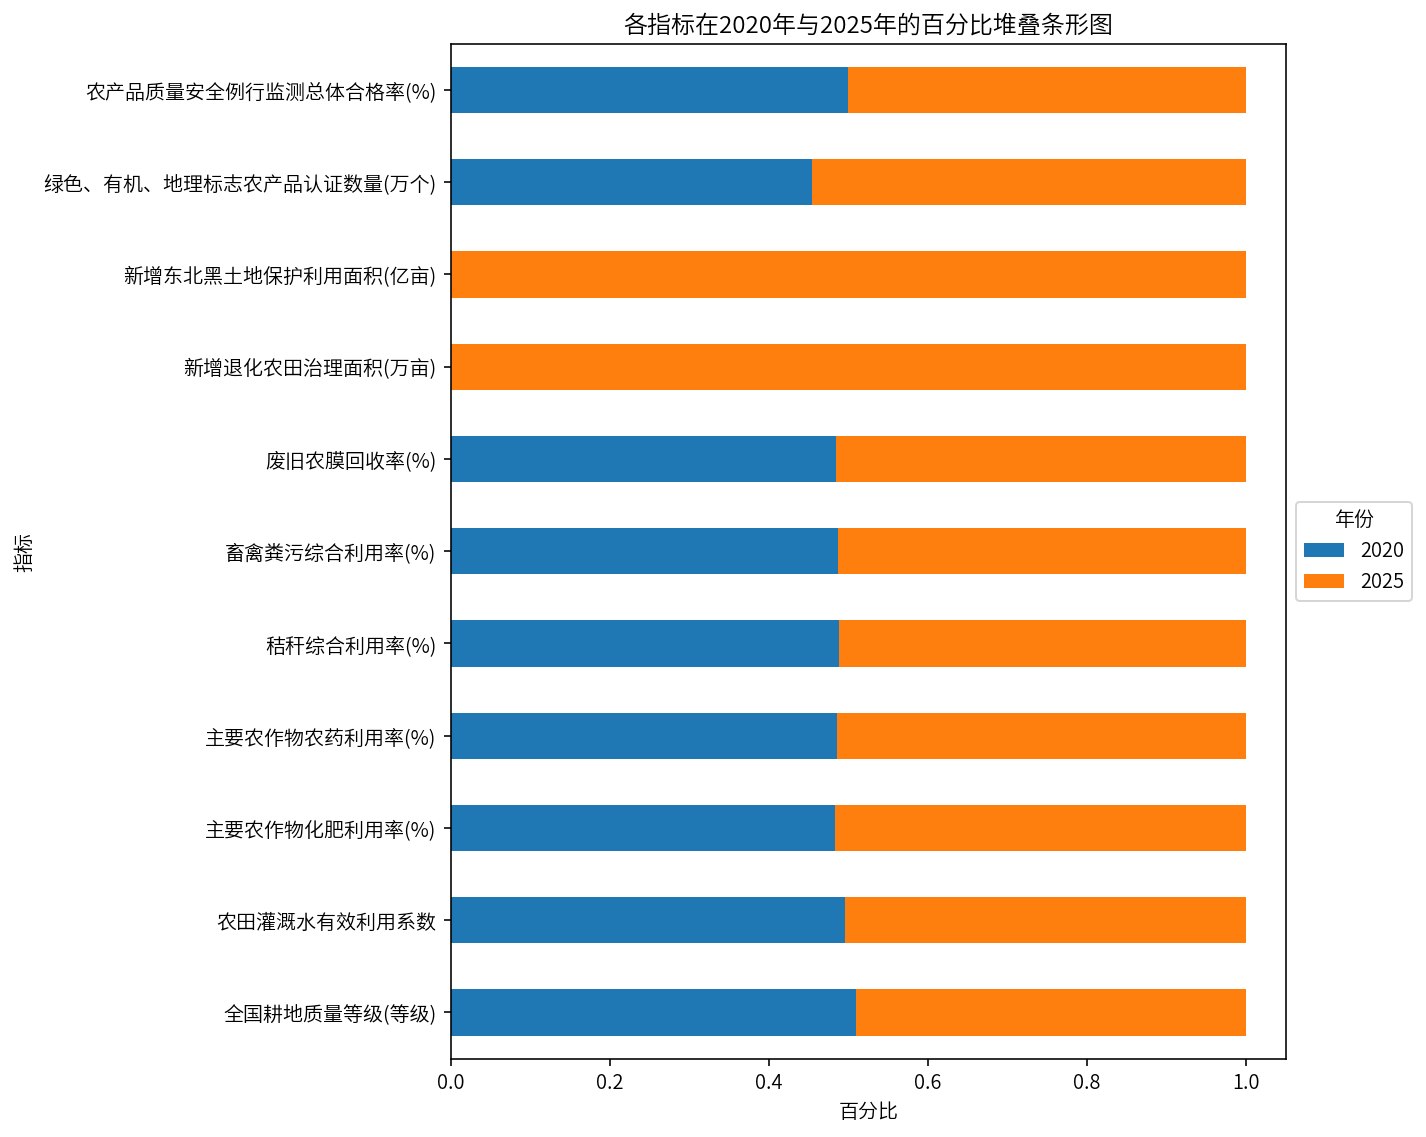
\includegraphics[width=0.7\linewidth]{figures/41.png}
    \caption{十四五规划流程目标图}
    \label{fig:enter-label}
\end{figure}

\section{科技对乡村农业的发展的影响}
\subsection{科技主要贡献}
农业现代化是实现可持续发展的关键,而农业科技现代化则是推动农业现代化的核心。本文综合收集并分析了农业科技在全国范围内的核心指标,涵盖农业科技进步贡献率、化肥与农药的有效利用率,以及县域数字农业发展的现状。依据这些关键指标,搜集了相应的数据,并据此绘制了热力图,如下图所示:

\begin{figure}[H]
    \centering
    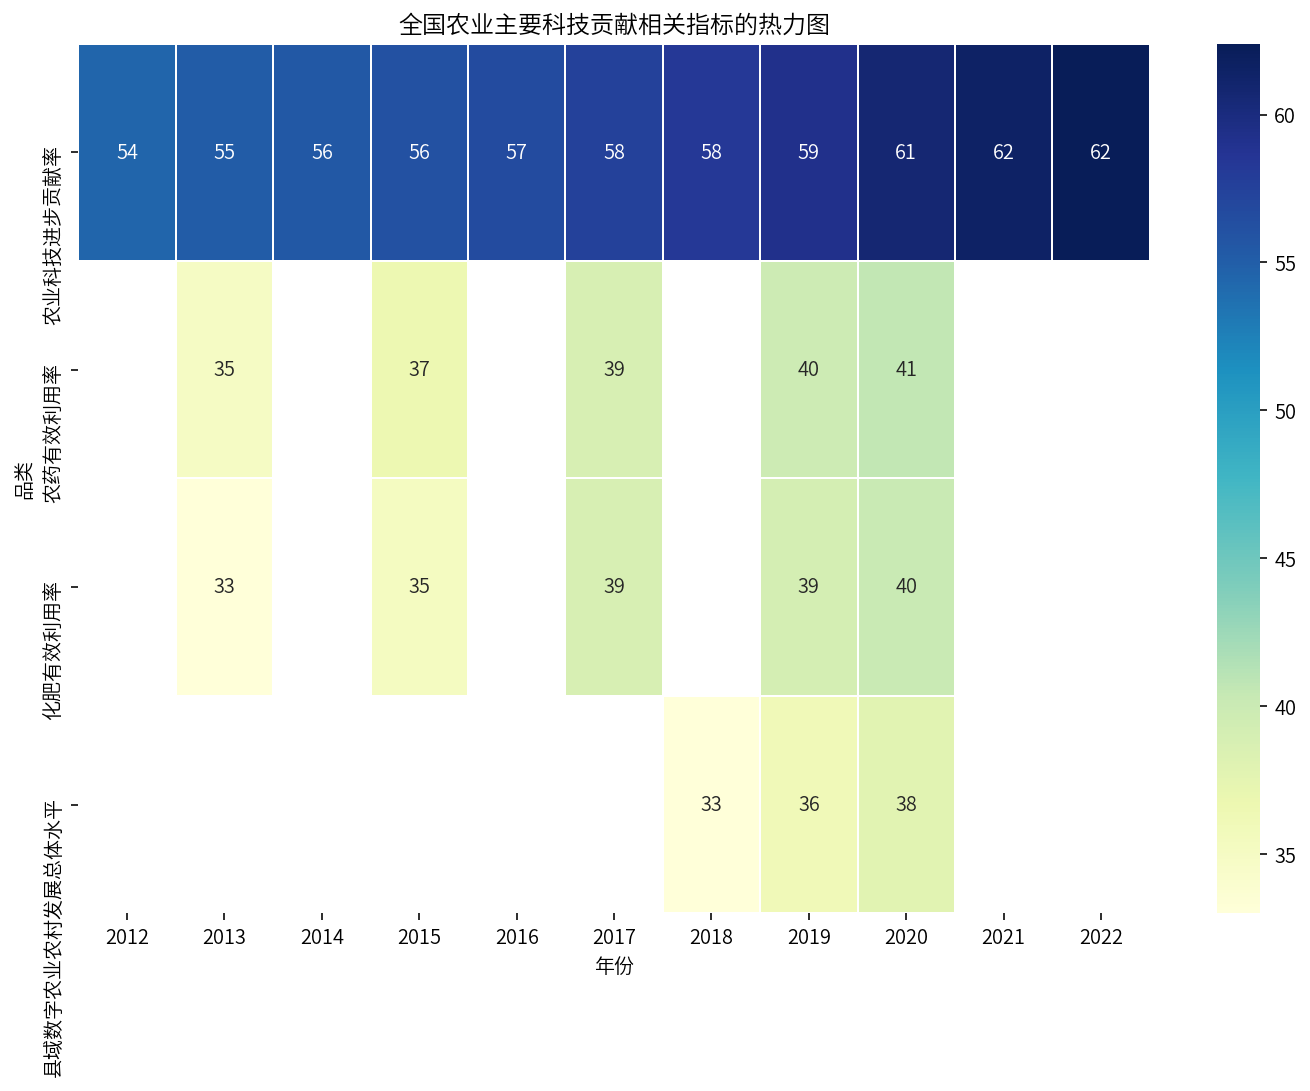
\includegraphics[width=0.5\linewidth]{figures/12.png}
    \caption{全国农业主要科技贡献相关指标的热力图}  
    \label{fig:Technology_hot}
\end{figure}

由图可知,科技在农业中的贡献逐年上升,体现在农业科技进步贡献率的持续增长。这不仅意味着科技创新在提高农业生产力方面起到了关键作用,而且反映出乡村经济正逐渐向技术密集型发展模式转变。

化肥和农药的有效利用率的增加,指向了农业生产过程中资源利用效率的提高。县域数字农业农村发展总体水平的提升也标志着信息技术在乡村振兴中的日益重要性,表明数字化转型在助力农业现代化和乡村经济发展中发挥着增效作用。
\subsection{数字农业渗透率}
随后,本文特别关注了数字农业渗透率这一关键指标,以评估技术如何在实际农业生产中得到应用并推动乡村经济的发展,绘制出如下的条形图\cite{china-digital-inclusion-development-report-2022}:

\begin{figure}[H]
    \centering
    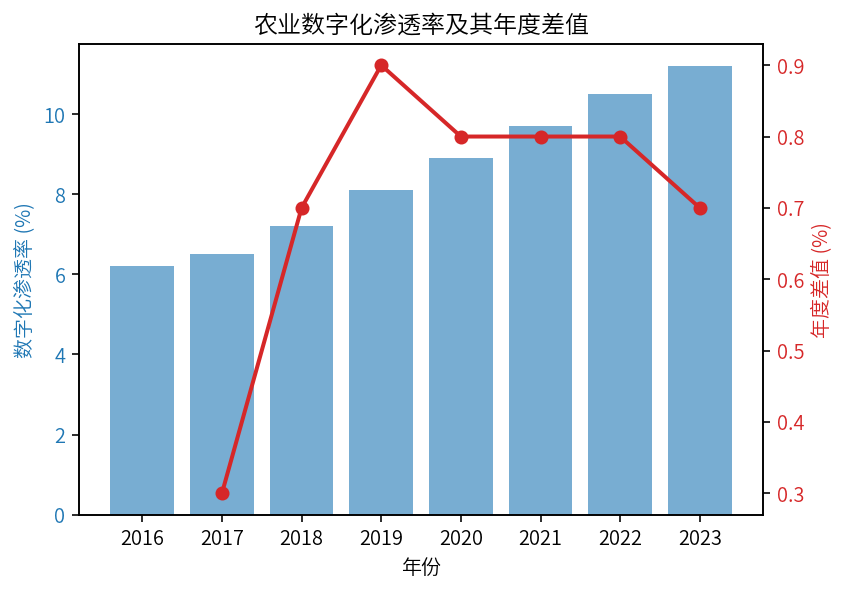
\includegraphics[width=0.6\linewidth]{figures/image1.png}
    \caption{数字农业渗透率折线图}
    \label{fig:Digital_agriculture_penetration}
\end{figure}

根据图表,可以看到农业数字化渗透率从2016年的0.062逐年增长,到2023年达到了0.112。从数字农业渗透率的变化趋势来看,数字化在农业中的应用呈现出逐年增长的态势,说明越来越多的农业生产活动正在通过数字技术进行优化和改进。

在本文中,采用了DLF-LSTM模型来对农业数字化渗透率进行建模和预测。在进行了详尽的测试之后,发现当学习率设置为0.004且经过100次迭代后,模型的损失率降至0.00138,并逐渐趋于稳定,这表明该模型达到了较高的预测精度。下面展示的图形描绘了模型训练过程中损失率的变化趋势,从中可以直观地观察到模型优化的效果和损失率随迭代次数的下降情况。

\begin{figure}[H]
    \centering
    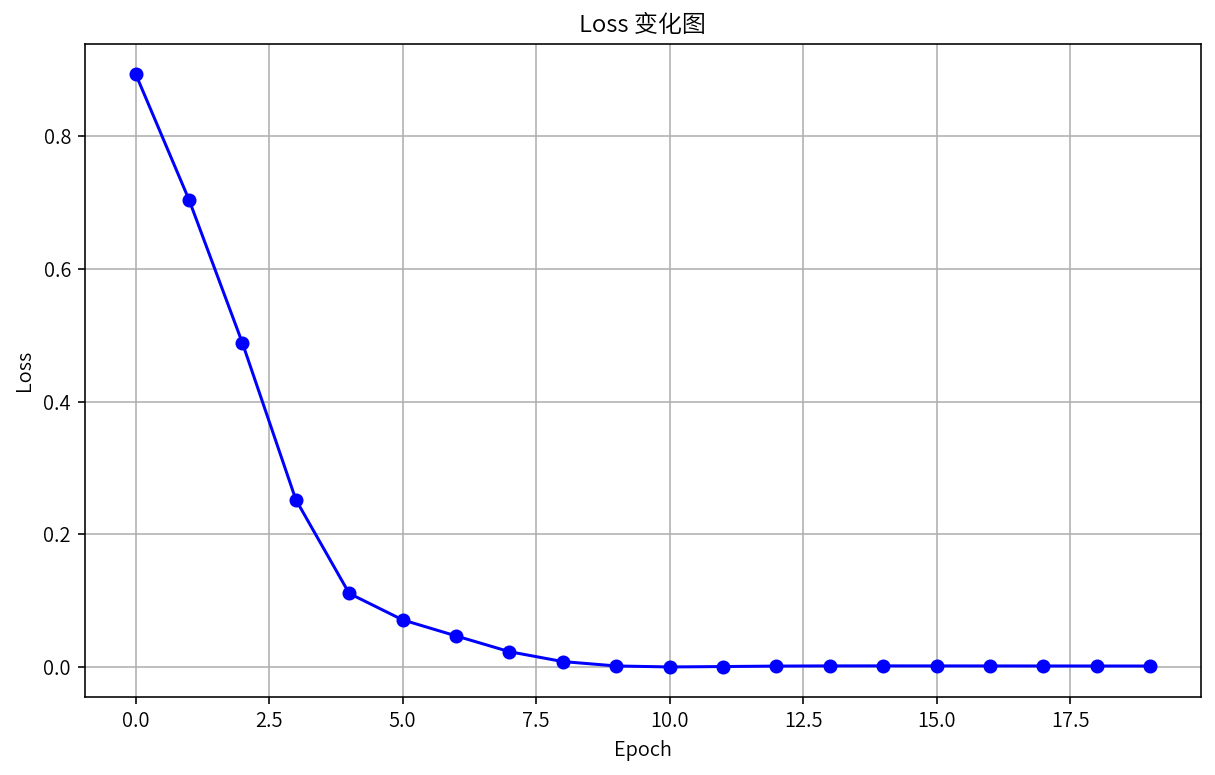
\includegraphics[width=0.65\linewidth]{figures/45.png}
    \caption{loss损失图}
    \label{fig:enter-label}
\end{figure}


预测数据如下表:
\begin{table}[H]
\caption{农业渗透话率预测表}
\centering
\begin{tabular}{cc}
\hline
\hline
\textbf{年份} &\textbf{预测农业渗透化率(万人)}\\
\hline
2024 & 0.12\\
2025 & 0.13\\
2026 & 0.14\\
2027 & 0.15\\
\hline
\end{tabular}
\end{table}

从预测数值来看,农业数字化渗透率在未来几年将保持稳步增长的态势。从2021年的0.12逐步增长到2027年的0.15,虽然整体呈现出向上的趋势,但增长幅度不是很大,且普及程度尚未达到预期的高水平。因此,可能需要进一步加大力度,推动数字技术在农业和乡村地区的广泛应用,以实现数字农业的全面渗透,带动乡村经济的全面发展。

\subsection{农业机械总动力}
在当前农业现代化的大背景下,农业机械化的推进尤显重要。本文借助国家统计局提供的权威数据,深入分析了我国农业机械化的发展态势。农业机械总动力,作为衡量农业机械化水平的重要指标,反映了全部农业机械动力的综合实力。绘制如下条形图进行分析:

\begin{figure}[H]
    \centering
    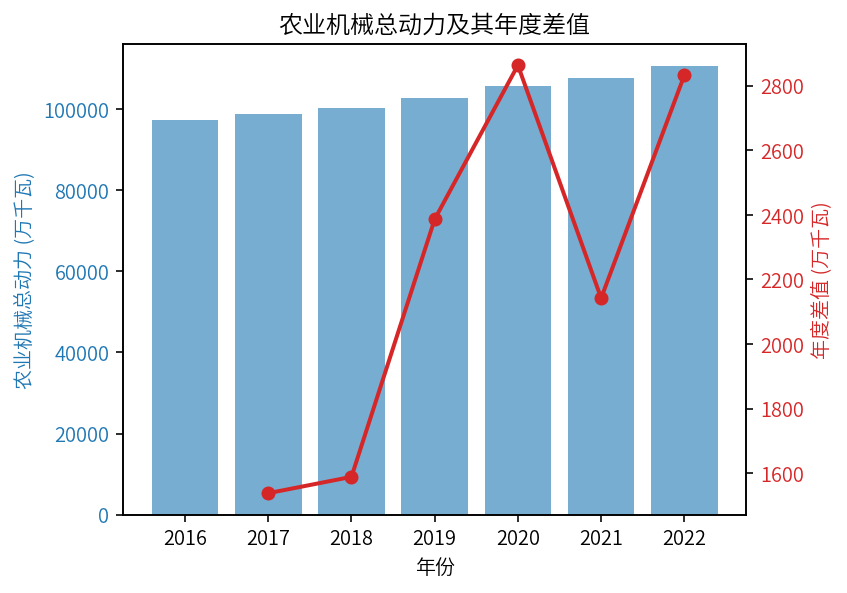
\includegraphics[width=0.6\linewidth]{figures/32.png}
    \caption{农业机械总动力条形图}
    \label{fig:agricultural_machinery_power}
\end{figure}

数据显示,我国农业机械总动力呈持续上升趋势。截至2022年,该指标达到了110597.19万千瓦,较去年增长了2800多万千瓦,展现了我国农业机械化快速发展的势头。

利用时间序列预测模型,进一步预测了未来的发展趋势。模型显示,若当前发展势头保持不变,农业机械总动力有望在未来几年内达到114378.54万千瓦。农业机械总动力的逐年提升,不仅彰显了国家在农机装备产业转型升级方面的坚定决心,也体现了农业农村部在推进“十四五”全国农业机械化发展规划中的积极作用\cite{china-digital-rural-development-2022}。
\begin{table}[H]
\caption{农业机械化预测表}
\centering
\begin{tabular}{cc}
\hline
\hline
\textbf{年份} &\textbf{未来农业机械总动力(万千瓦)}\\
\hline
2023 & 114378.54\\
2024 & 117931.49\\
2025 & 121980.57\\
\hline
\end{tabular}
\end{table}
农业机械化的持续发展是国家现代化农业战略的重要组成部分。随着政府对农业机械化的持续投入和政策支持,有理由相信,我国农业机械化的未来将更加光明,为实现乡村振兴战略贡献更大的力量。

\section{科技对乡村居民生活的影响}

随着我国乡村振兴战略的深入实施,科技创新力量不断渗透到乡村生活的各个层面,显著改变了广大农村居民的日常生活习惯和经济社会发展面貌。近年来,国家积极推动互联网基础设施向农村延伸,加快缩小城乡数字鸿沟,这一举措成效显著。

\begin{figure}[H]
    \centering
    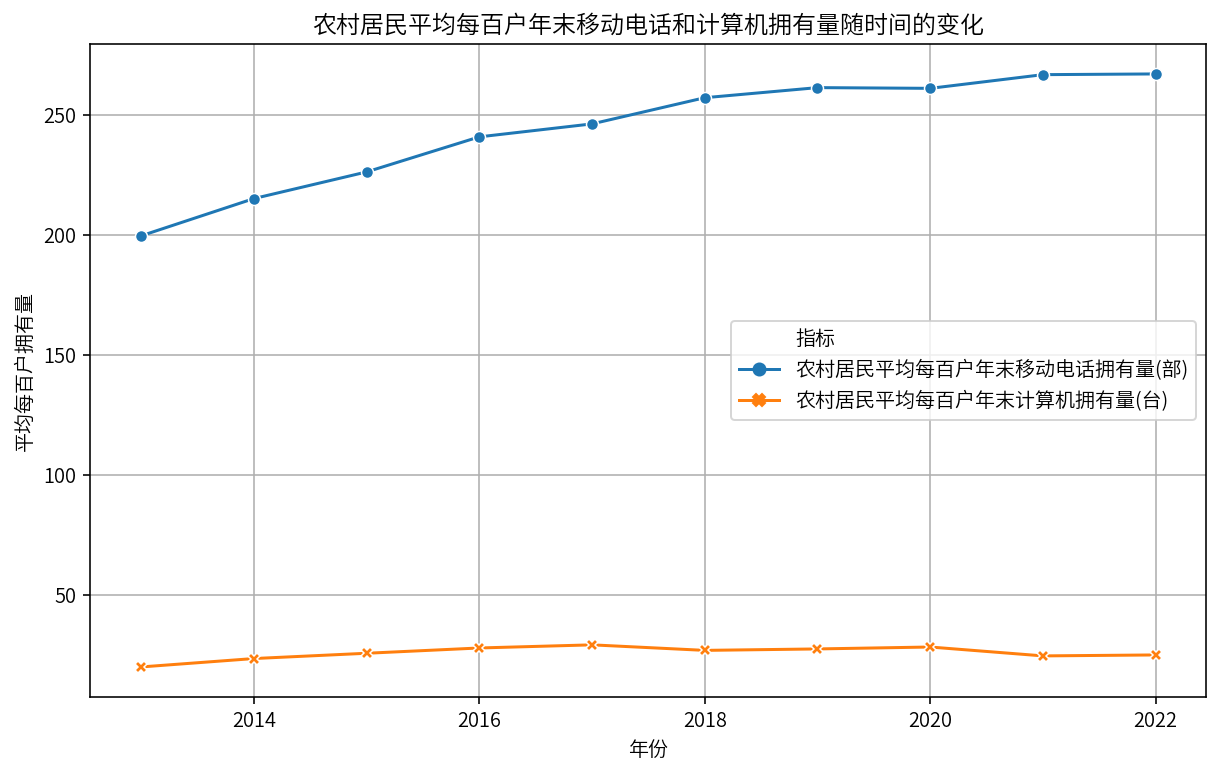
\includegraphics[width=0.65\linewidth]{figures/42.png}
    \caption{电子设备使用量序列图}
    \label{fig:enter-label}
\end{figure}

本文通过绘制时间序列的折线图,进而揭示了农村居民对电脑和手机这两类主要电子设备的使用趋势。随着互联网技术的广泛普及,可以观察到农村居民的手机拥有量呈现出显著的增长趋势,反映了移动设备在日常生活中的重要地位。相对而言,电脑的使用量在这段时间内变化不大,暗示着农村地区对于电脑的需求和应用场景仍然有限,或许是由于农村地区对高科技设备的适应性和接受度有待提高。

通过对城乡居民互联网使用状况的数据分析可以发现,无论是城市还是乡村,互联网普及率均呈现出稳步上升的趋势。特别是在过去几年间,随着移动互联网技术的普及和网络资费的下调,越来越多的农村居民得以接入互联网,享受到便捷高效的数字化服务\cite{digital-village-strategy}。

\begin{table}[H]
    \centering
    \caption{2020-2022城乡居民互联网使用量预测}
    \begin{tabular}{ccc}
        \hline
        \hline
        \textbf{年份} &\textbf{农村居民互联网使用量预测}&\textbf{城镇居民互联网使用量预测}\\
        \hline
        2020&63.680962&77.475733\\
        2022&82.730215&98.743864\\
        \hline
    \end{tabular}
    \label{tab:Internet}
\end{table}

本数据缺失2020到2022的数据,因此使用指数平滑法进行预测。结合趋势推测,当前城乡互联网用户的比例可能接近于5:4这样一个水平,预示着乡村互联网市场潜力巨大,并有望在未来进一步激活农村经济,助力乡村振兴战略目标的实现。

\begin{figure}[H]
    \centering
    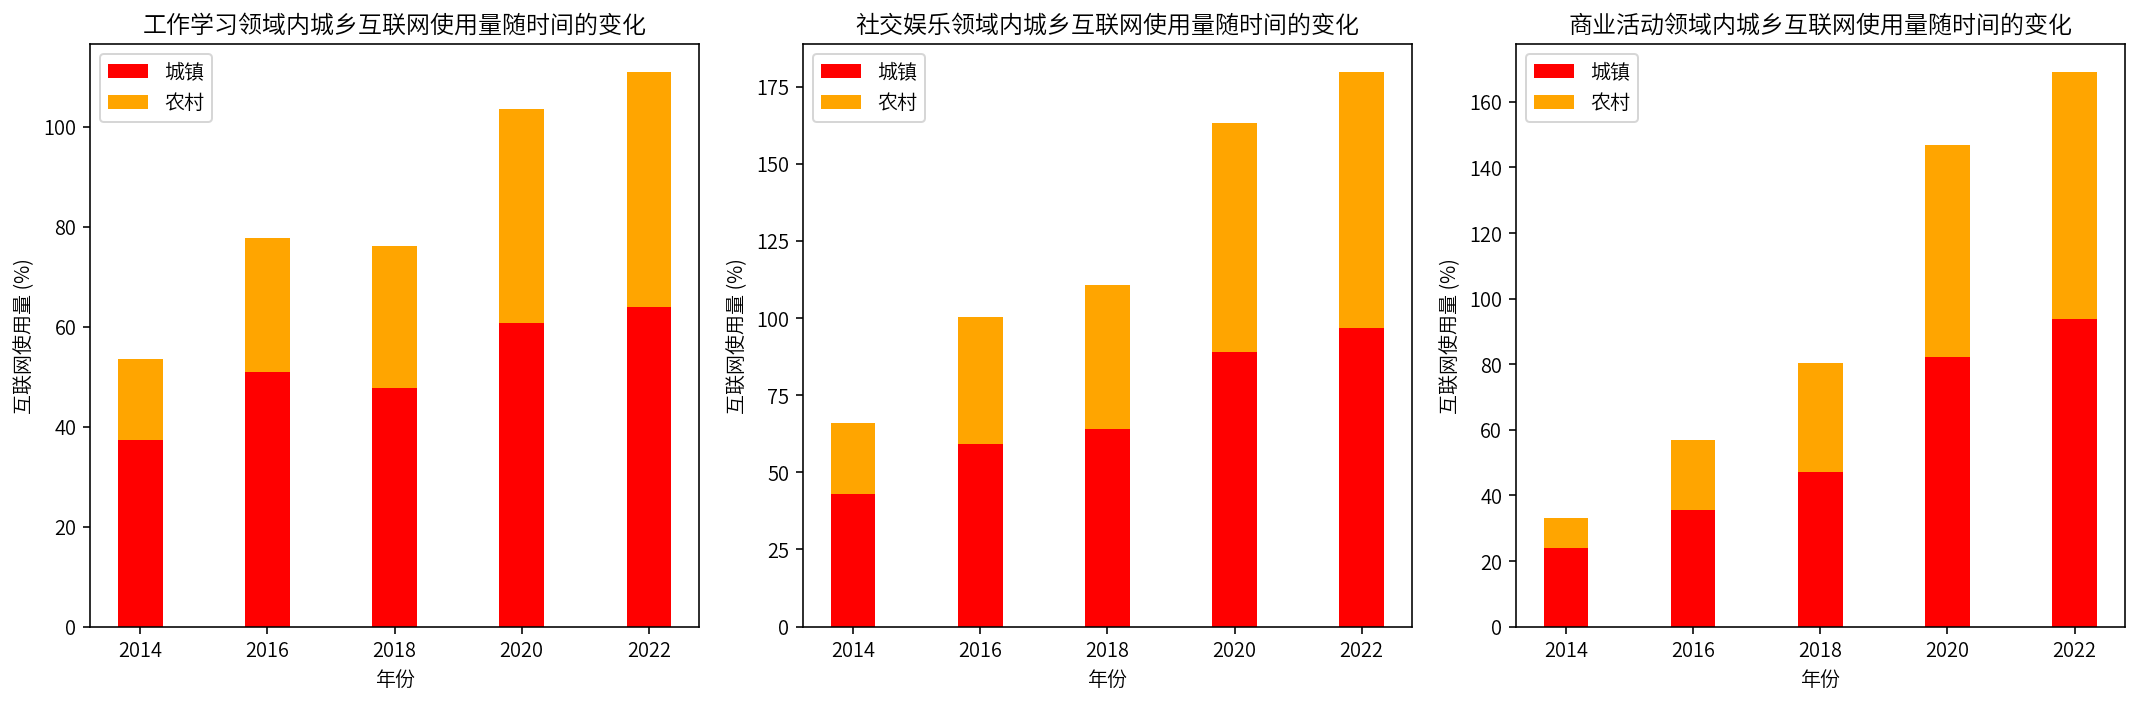
\includegraphics[width=1\linewidth]{figures/50.png}
    \caption{城乡互联网使用量随时间变化对比图}
    \label{fig:enter-label}
\end{figure}

数据显示,城乡间的互联网使用量差距正在逐年缩减。农村地区的互联网普及率不断提升,尤其是在商务交易、网络支付、信息获取等方面的应用率增长明显,这表明农村居民正加速融入数字经济的大潮之中。例如,农村网民通过电商平台进行农产品销售、利用网络平台开展技能培训、借助移动支付实现无现金交易等活动日益普遍。


这些数据共同映射了中国乡村经济在科技推动下的积极变化,揭示了科技进步是乡村振兴策略的关键驱动力。